% Created 2024-10-10 Thu 17:04
% Intended LaTeX compiler: pdflatex

        \documentclass[10pt]{article}
\usepackage[T1]{fontenc}
\usepackage[utf8]{inputenc}
\usepackage[swedish, english]{babel}
\usepackage{amsfonts,amsmath,amssymb}
\usepackage{/home/john/Documents/skola/tex/old_notestex_en}

    \usepackage[T1]{fontenc}     
    \usepackage[utf8]{inputenc} 
    \usepackage[swedish]{babel}
    \usepackage{amsfonts}
    \usepackage{amsmath}
    \usepackage{amssymb}
    \usepackage{hyperref}
    \newcommand\NN{\ensuremath{\mathbb{N}}}
    \newcommand\RR{\ensuremath{\mathbb{R}}}
    \newcommand\ZZ{\ensuremath{\mathbb{Z}}}
    \renewcommand\O{\ensuremath{\\emptyset}}
    \newcommand\QQ{\ensuremath{\mathbb{Q}}}
    \newcommand\CC{\ensuremath{\mathbb{C}}}
    \usepackage{import}
    \usepackage{xifthen}
    \usepackage{pdfpages}
    \usepackage{transparent}

    \newcommand{\incfig}[1]{%
        \def\svgwidth{\columnwidth}
        \import{./img/}{#1.pdf_tex}
    }
\usepackage[utf8]{inputenc} 

\usepackage[T1]{fontenc} 

\usepackage{amsmath} 

\usepackage{amssymb} 

\usepackage{enumerate} 

\usepackage{prftree} 

\usepackage{mathpartir} 

\usepackage{mathtools} 

\usepackage{stmaryrd} 

\usepackage{color} 

\definecolor{darkgreen}{rgb}{0,0.45,0} 

%\usepackage[colorlinks,urlcolor=darkgreen,linkcolor=darkgreen]{hyperref} 

\makeatletter 

\newlength{\tempwidth@narrowinferruleconcl} 

\newcommand{\narrowinferrule}[4][0pt]{% 

  % Optional argument #1: optional extra padding 

  % Compulsory arguments #2–#4: arguments of \inferrule* (but optional arg of that is compulsory here) 

  \settowidth{\tempwidth@narrowinferruleconcl}{$#4$}% width of conclusion 

  \mathmakebox[\tempwidth@narrowinferruleconcl+#1][c]% 

    {\inferrule*[right=\protect{\rlap{#2}}]{#3}{#4} \hspace*{-1.4ex}}%  

  } 

 

\newcommand{\negphantom}[1]{\settowidth{\dimen0}{#1}\hspace*{-\dimen0}} 

\makeatother 

 

\newcommand{\todo}[1]{\textcolor{red}{#1}} 

 

% styled letters 

\newcommand{\A}{\mathcal{A}} 

\newcommand{\D}{\mathcal{D}} 

\newcommand{\N}{\mathbb{N}} 

\newcommand{\cN}{\mathcal{N}} 

\newcommand{\R}{\mathbb{R}} 

\newcommand{\cR}{\mathcal{R}} 

\newcommand{\Z}{\mathbb{Z}} 

\newcommand{\V}{\mathcal{V}} 

\newcommand{\Q}{\mathbb{Q}} 

\newcommand{\cQ}{\mathcal{Q}} 

% binary relations 

\newcommand{\proves}[1][]{\mathrel{\vdash_{#1}}} 

\newcommand{\notproves}[1][]{\mathrel{\nvdash_{#1}}} 

\newcommand{\entails}[1][]{\mathrel{\vDash_{#1}}} 

\newcommand{\notentails}[1][]{\mathrel{\nvDash_{#1}}} 

\newcommand{\believes}[1][]{\mathrel{\vDash_{#1}}} 

\newcommand{\notbelieves}[1][]{\mathrel{\nvDash_{#1}}} 

\newcommand{\logequiv}{\approx} 

 

% syntax of logic 

\newcommand{\limp}{\rightarrow} 

\newcommand{\liff}{\leftrightarrow} 

\newcommand{\ltrue}{\top} 

\newcommand{\lfalse}{\bot} 

\renewcommand{\land}{\wedge} 

 

% miscellaneous 

 

\renewcommand{\Form}{\mathrm{Form}} 

\newcommand{\Term}{\mathrm{Term}} 

 

\newcommand{\signature}[1]{\langle\, #1\, \rangle} 

\newcommand{\strux}[1]{\langle\, #1\, \rangle} 

\newcommand{\nextpart}{\,\mathpunct{;}\,} 

\newcommand{\interp}[2][]{\llbracket\; #2\; \rrbracket^{#1}}
\author{Typeset by John Möller}
\date{\today}
\title{Lecture 9 notes // Statistical Methods}
\hypersetup{
 pdfauthor={Typeset by John Möller},
 pdftitle={Lecture 9 notes // Statistical Methods},
 pdfkeywords={},
 pdfsubject={},
 pdfcreator={Emacs 29.4 (Org mode 9.6.15)}, 
 pdflang={English}}
\begin{document}

\title{{Lecture 9 notes}\\{\normalsize{\itshape Statistical Methods}}}
\pagestyle{fancynotes}
\maketitle
\section{MVUE}
\label{sec:orgb0d0440}
Minimal Variance Unbiased Estimator (MVUE):

\begin{theorem}[Lehman-Schally] \label{thm:Lehman-Schally}
Let \(T(X_1, \dots , X_n)\) be an unbiased estimator of \(g(\theta )\).

\begin{align*}
E(T(X_1 , \dots , X_n)) =  g(\theta )
\end{align*}
with finite variance.
T is MVUE for \(\theta\) iff \(E(T(X_1, \dots , X_n) = S(X_1 , \dots , X_n)) =  0\) for every \(S\) s.t. \(E(S(X_1 , \dots , X_n )) =  0\),
\(\text{Var}(S) < \infty\),
we can use "special estimators" ex BLUE (Best linear unbiased estimator) in lin reg MSE is usually BLUE.
CDF:
\begin{align*}
F(x) =  P( X \leq x)
\end{align*}
\end{theorem}

\begin{definition}[Empirical cumulative distribution function]  \label{def:Empirical_cumulative_distribution_function}
\begin{align*}
F_n (u, (X_1, \dots , X_n)) =  n  ^{ - 1} \sum_{ i = 0 }^{ n } I  _{( - u, u)} (X_i)  &  =
\begin{cases}
0,  &  u \leq X _{(1)} \\
\frac{k}{n} X  _{(k)}  \leq u \leq  X  _{k + 1} \\
1  &  u > X  _{(n)} .
\end{cases}
\end{align*}
\end{definition}

\section{Order statistics}
\label{sec:orgaf8312e}
\begin{align*}
X_1 , \dots , X_n  \Rightarrow X  _{(1)} \leq X _{(2)} \leq \dots \leq X  _{(n)} 
\end{align*}
\begin{center}
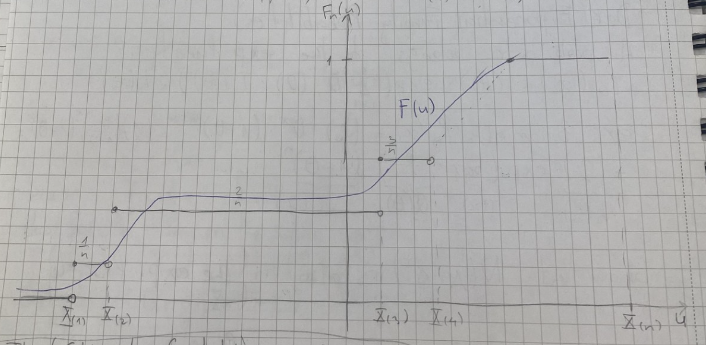
\includegraphics[angle=0,width=10cm]{./img/order.png}
\end{center}


\begin{theorem}[Glivenko-Conteli] \label{thm:Glivenko-Conteli}
\begin{align*}
F_n \rightarrow F
\end{align*}
as \(n \rightarrow \infty\) "in some sense".
\end{theorem}



\begin{align*}
 &  X_i \sim \text{N}(\mu , \sigma^2) \\
 &  \overline{X} \sim N(\mu  \frac{\sigma ^2 }{n} \\
 &  \frac{\overline{X} -  \mu }{\frac{\sigma}{\sqrt{n}}} \\
 &  \text{ Show: } \\
 &  \overline{X} \pm \epsilon 
\end{align*}

\begin{align*}
P( - 1.96 \leq \frac{\overline{X} - \mu }{\frac{\sigma }{\sqrt{n}}} \leq 1.96)  &  =  95 \%  / -  \frac{\sigma}{\sqrt{n}} \\
P( - 1.96  \frac{\sigma }{\sqrt{n}}\leq \overline{X} - \mu \leq 1.96 \frac{\sigma }{\sqrt{n}})  &  =  95 \%  / -  \overline{X} \\
P( - 1.96  \frac{\sigma }{\sqrt{n}} - \overline{X} \leq - \mu \leq 1.96 \frac{\sigma }{\sqrt{n}} - \overline{X})  &  =  95 \%  / -  ( - 1) \\
P( \overline{X} - 1.96  \frac{\sigma }{\sqrt{n}}  \leq  \mu \leq \overline{X} + 1.96 \frac{\sigma }{\sqrt{n}})  &  =  95 \%.
\end{align*}
\begin{center}
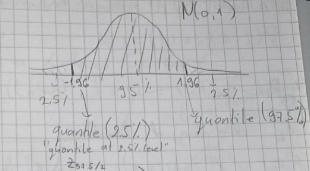
\includegraphics[angle=0,width=10cm]{./img/bell.png}
\end{center}

\begin{definition}[Quantile]  \label{def:Quantile}
\(z _{\alpha }\) is defined as to satisfy the following equation:
\begin{align*}
P(z \geq z _{\alpha } ) = \alpha .
\end{align*}
\end{definition}


\begin{definition}[Confidence Interval]  \label{def:Confidence_Interval}
A RANDOM interval \((L,U)\)

\([L,U]\) is a confidence interval for parameter \(\theta\) with confidence level \(\alpha\) if
\begin{align*}
P(L \leq \theta \leq U) =  1 - \alpha
\end{align*}

Confidence interval \((L,U)\) covers \(\theta\) with \(1 - \alpha\) probability.
\end{definition}



\begin{align*}
\overline{X} \pm z  _{\frac{\alpha}{2}} \cdot \frac{\sigma }{\sqrt{n}}
\end{align*}
is a \(\alpha\)-level confidence interval for \(\mu\).

\begin{exercise}[]  \label{exe:}
\begin{center}

\includegraphics[angle=0,width=5cm]{./img/exe1.png}
\end{center}
\end{exercise}


\begin{exercise}[]  \label{exe:}
Show
\(( - \infty , \overline{X} + Z  _{\frac{\alpha}{2}} \frac{\sigma}{\sqrt{n}})\) and
\((\overline{X} -  Z _{\frac{\alpha}{2}} \frac{\sigma}{\sqrt{n}}, \infty)\) are also \((1 - \alpha )\)-confidence intervals for \(\mu\).
\end{exercise}

\begin{exercise}[]  \label{exe:}
Show sizes of confidence intervals.
\end{exercise}



\textbf{"Statistic:"}
\(H _{\theta }  = h(\text{ data }, \theta )\), with a known distribution.

\(P( L \leq H _{\theta } \leq U) = 1 - \alpha\).

\textbf{Fact:}
If \(X_i \sim \text{N}(0 , 1)\) and \(Y =  X_1 ^2 + \dots + X_n^2\) then
\(Y \sim \chi  _{k} ^2\) where \(k\) is the degrees of freedom.

Let \(X_i \sim \text{N}(\mu , \sigma^2)\). Since \(\frac{X_i -  \mu }{\sigma } \sim \text{N}(0 , 1)\) that means
\begin{align*}
\sum_{ i = 1 }^{ n } \frac{\left( X_i - \mu  \right) ^2 }{\sigma ^2 } \sim \chi ^2  _{n} .
\end{align*}

"More difficult:"
\begin{align*}
\sum_{ i = 1 }^{ n } \frac{(X_i -  \overline{X}) ^2 }{\sigma ^2 } \sim \chi  _{n - 1} ^2 .
\end{align*}


\begin{definition}[Sample Variance]  \label{def:Sample_Variance}
\begin{align*}
s ^2  &  = \sum_{ i = 1 }^{ n } \frac{(X_i - \overline{X})^2 }{n - 1}
\end{align*}
\end{definition}

Thus:

\begin{theorem}[] \label{thm:}
\begin{align*}
\frac{n - 1}{\sigma ^2 } s^2  \sim \chi  _{n - 1} ^2 .
\end{align*}
\end{theorem}

Quantile of \(\chi  _{n} ^2\) of \(1 - \alpha\) level \(\chi ^2  _{\alpha } (n)\) is a point s.t.
\(P(Y \geq \chi  _{\alpha } ^2 (n)) = \alpha\), \(Y \sim X _{n} ^2\)

\begin{center}
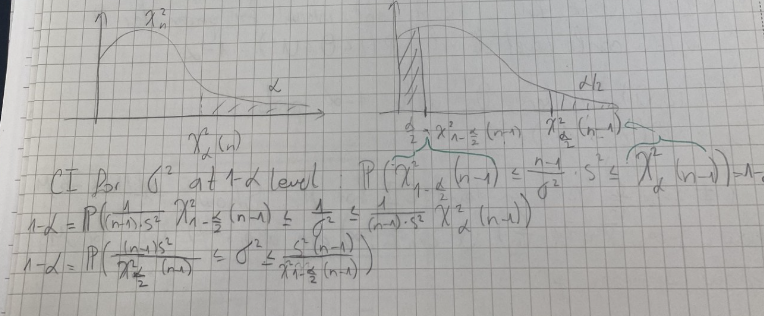
\includegraphics[angle=0,width=10cm]{./img/chi.png}
\end{center}


\begin{theorem}[] \label{thm:}
Let \(X_1, \dots , X_n\) be on i.i.d sample from \(\text{N}(\mu , \sigma^2)\), where
\(\mu\) and \(\delta\) are unknow, then,
\begin{align*}
\left[ \frac{(n - 1) \cdot s^2 }{\chi  _{\frac{\alpha}{2}}(n - 1) }, \frac{(n - 1) s ^2 }{\chi  _{1 - \frac{\alpha}{2}} (n - 1)} \right] 
\end{align*}
is an \(\alpha\)-level confidence interval for \(\sigma ^2\).
\end{theorem}

Let \(X_i \sim \text{N}(\mu , \sigma^2)\) then
\begin{align*}
\frac{\overline{X} - \mu }{s / \sqrt{n}} \sim t(n - 1)
\end{align*}
where \(s = \sqrt{s^2 }\).

\begin{exercise}[]  \label{exe:}
Show \(\overline{X} \pm t _{\alpha  / 2} (n - 1) \cdot \frac{s}{\sqrt{n}}\) is a \(1 - \alpha\) level quantile for \(\mu\).
\end{exercise}


\section{Statistical Hypothesis Testing}
\label{sec:org143dc20}


\begin{align*}
H_0 :  &  \mu = \mu  _{0}  \\
H_1 :  &  \mu \neq \mu  _{0} 
\end{align*}

Construct a test statistic
\begin{align*}
T = T(X_1, \dots , X_n | H_0) \sim \tilde{f}(\mu  _{0} ).
\end{align*}

\begin{align*}
X_1, \dots , X_n
\end{align*}
is a random sample

\begin{align*}
T(X_1 , \dots , X_n) \in  \text{ critical set } \theta  _{1} 
\end{align*}

If \(T \in  \theta  _{1}\) then we reject the null hypothesis.

If \(T \not\in \theta  _{1}\) then we fail to reject the null hypothesis.

\begin{align*}
P(T \in  \theta  _{1}  | H_0 \text{ is true }) = \alpha .
\end{align*}
\end{document}
